% !Mode:: "TeX:UTF-8"

\titlecontents{chapter}[2em]{\vspace{.5\baselineskip}\xiaosan\song}
             {\prechaptername\CJKnumber{\thecontentslabel}\postchaptername\qquad}{}
             {}             % 设置该选项为空是为了不让目录中显示页码
\addcontentsline{toc}{chapter}{中文译文}
\setcounter{page}{1}            % 单独从 1 开始编页码
\markboth{中文译文}{中文译文}   % 用于将章节号添加到页眉中
%\captionsetup[figure]{labelfont={bf},labelformat={default},labelsep=period,name={Fig.}}
%\chapter*{中文译文}

\trtitle{FlowNet2: }
\trabs{摘 \qquad 要}
\par\setlength{\parindent}{2em} FlowNet 证明光流估计可以被看作是一个学习问题。然而,传统方法在光流质量方面仍然是现在最先进的方法,特别是在小位移和真实数据中,FlowNet不能与变量的方法相比。在这篇论文中,我们发展了端对端光流估计的概念,并且使此概念有很好的效果。在质量和速度方面的提升主要源于三个方面:首先,我们关注训练数据,发现载入数据的顺序安排很重要;第二,我们研究了一个堆叠的结构,包括用中间阶段的光流变化第二张图片;第三,通过引入一个关于小运动的子网络,我们在小位移上进行了详细操作。FlowNet 2.0 只比FlowNet慢一点,但是在错误率方面减少超过50\%。这个方法可以与最先进的方法相提并论,并且以交互式码率运行。此外,我们提出了更快的变体,计算效率高达140fps,而且与最初的FlowNet的准确率相当。
\begin{figure}[h]
	\centering
	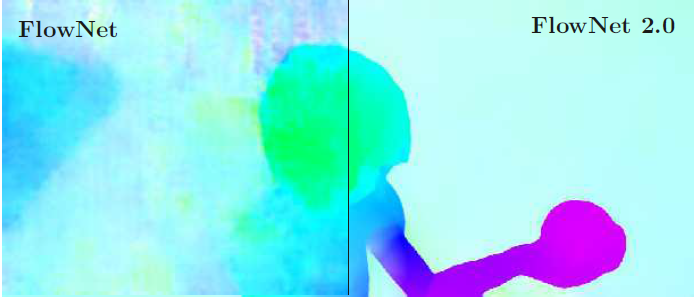
\includegraphics[width=1\textwidth]{figures/translate/1.png}
	\caption{我们提出的FlowNet的进化版本。FlowNet2.0能有更平滑的光流场,能够保持很好的运动细节,并且以8到140fps的速度运行。这个示例中,FlowNet2.0的准确率是最初FlowNet的四倍}
	\label{fig1}
\end{figure}


\trchapter{1.介绍}

Dosovitskiy et al. \cite{dosovitskiy2015flownet} 提出的FlowNet表现了光流估计问题的范式转变。使用一个简单的卷积神经网络结构直接从数据中学习光流的概念的思想与所有现有的方法都不相同。然而,新想法的首次实现往往很难与高度优化的现有的方法相提并论,FlowNet也不例外。接连的巩固解决了这些负面的影响,使我们从新思路中受益。
\par
这篇论文是FlowNet的巩固。FlowNet2.0继承了FlowNet的优点,例如,掌控大位移,正确预测光流场中的细节,对于具体问题有学习先验的潜力,以及快速的运行速度。同时,FlowNet2.0解决了小位移以及光流场中的噪声失真问题。这些进步使得FlowNet2.0在真实世界应用上有了很大的提升,例如行为识别和运动分割,使得FlowNet2.0达到了最先进的水平。
\par
几个渐进但是决定性的变化导向了FlowNet2.0,虽然这些变化并不是完全与观察到的问题相连。首先,我们评价了数据集安排的影响。有趣的是,Mayer et al \cite{Mayer2016A} 提出的越复杂的数据集,单独使用时结果越差。然而,包括各种数据集的学习策略可以极大地提升准确率。在这个范围内,我们也发现FlowNet使用显式互相关层的版本比没有这一层的版本表现得更好,这与Dosovitskiy et al. \cite{dosovitskiy2015flownet}提出的结果相反。
\par
第二个贡献是,我们引入了变形操作,并且展示了堆叠网络使用这个操作可以很有效的提升结果。通过变化堆叠深度以及单独组成部分的尺寸,我们获得了许多有着不同尺寸和运行时间的网络变体。这允许我们权衡计算资源和准确率。我们提供频率在8fps到140fps的网络。
\par
最后,我们专注于小的,半像素的运动和真实世界数据。为此目的,我们创造了一个特别的训练数据集和一个专门的网络。我们展示了用这个数据训练的结构在真实世界视频典型的小运动上表现得很好。为了达到在任意位移上最优的表现,我们增加了一个网络,这个网络以一个最优的方式融合之前堆叠的网络和小位移网络。
\par
最终的网络性能超越了FlowNet很多,并且在Sintel和KITTI数据集上可以与最先进的方法相提并论。这个方法可以很细节的估计小的和大的位移,并且提供交互式的帧率。










